% use paper, or submit
% use 11 pt (preferred), 12 pt, or 10 pt only

%\documentclass[letterpaper, preprint, paper,11pt]{AAS}	% for preprint proceedings
\documentclass[letterpaper, paper,11pt]{AAS}	
%\setcounter{secnumdepth}{3}	% for final proceedings (20-page limit)
%\documentclass[letterpaper, paper,12pt]{AAS}		% for final proceedings (20-page limit)
%\documentclass[letterpaper, paper,10pt]{AAS}		% for final proceedings (20-page limit)
%\documentclass[letterpaper, submit]{AAS}			% to submit to JAS

\usepackage{bm}
\usepackage{amsmath}
\usepackage{subfigure}
\usepackage{float}
\usepackage{circuitikz}
%\usepackage[notref,notcite]{showkeys}  % use this to temporarily show labels
\usepackage[colorlinks=true, pdfstartview=FitV, linkcolor=black, citecolor= black, urlcolor= black]{hyperref}
\usepackage{overcite}
\usepackage{footnpag}			      	% make footnote symbols restart on each page




\PaperNumber{16-451}



\begin{document}

\title{MINIMUM ENERGY, REACTION-WHEEL BASED, CUBESAT ATTITUDE CONTROL: A COMPARISON OF COST FUNCTIONS}

\author{Dmitriy Rivkin\thanks{Graduate Student, Department of Computer Engineering, UC Santa Cruz, Santa Cruz, CA, 95064.}  
%Qi Gong\thanks{Associate Professor, Department of Applied Mathematics and Statistics, UC Santa Cruz, Santa Cruz, CA, 95064.},
\ and Gabriel Elkaim\thanks{Professor, Department of Computer Engineering, UC Santa Cruz, Santa Cruz, CA, 95064.}
}


\maketitle{} 		


\begin{abstract}
A Legendre pseudospectral method is used to solve the minimum energy reorientation problem for a 3U Cubesat with three orthogonal reaction wheels. Optimization is performed with respect to a cost functional that represents battery energy losses, and includes terms arising from resistive losses in the armature resistance, friction in the bearings, and mechanical kinetic energy, which is unrecoverable in the absence of a regenerative braking system. To overcome numerical challenges associated with this cost functional, a novel approximation method is introduced. Results are compared with those obtained using the standard ``integral of control torque squared'' cost functional, and it is shown that, if the ratio between the moments of inertia of the satellite body and the reaction wheels is large, optimization with respect to the standard cost functional does not produce an energy-optimal solution.
\end{abstract}


\section{Introduction}
Cubesats are small satellites whose size and shape is referred to in terms of units. A three unit (3U) Cubesat has dimensions $10cm \times 10cm \times 30cm$ and a mass of about $3kg$. A Cubesat's only source of energy is its battery, which is recharged by solar panels covering the (very small) body. Therefore, Cubesats operate under severe energy constraints, which motivates the development of energy optimal attitude maneuvers. Reaction wheel based controllers are popular when the application requires high pointing accuracy and rapid reorientation because they do not require any fuel, consuming only electrical energy. Unlike larger satellites, which often have redundant, tetrahedral arrangements of reaction wheels, Cubesat attitude controllers usually have only three, orthogonally arranged, reaction wheels. This is due to severe weight constraints and the relatively low cost of replacing a malfunctioning satellite. Many of these reaction wheel arrays do not have regenerative braking, meaning the kinetic energy of the reaction wheels is unrecoverable. Most of the Cubesats with high performance, reaction wheel based controllers are 3U, because such a system in smaller satellites leaves insufficient room for payload. Therefore, this paper is concerned with computing electrical energy minimizing trajectories for a 3U Cubesat with three reaction wheels which are incapable of regenerative braking.

\subsection{Methods}
A Legendre pseudospectral method \cite{Ross2012} is applied to compute a state-control trajectory pair that minimizes a cost functional and satisfies dynamic constraints, as implemented by the software package DIDO\cite{Ross2007}. This method allows for optimization in the presence of non-linear dynamic constraints. The cost functional is derived by analysis of the power supplied by the battery and depends on applied torque and wheel speed, containing terms arising from three sources of energy loss: resistive losses in the armature resistance, friction in the bearings, and mechanical kinetic energy, which is unrecoverable in the absence of regenerative braking capabilities. This approach is computationally expensive, however, a precomputed energy optimal trajectory can be tracked by a closed loop controller. Karpenko \textit{et al} provide a practical implementation of the tracking controller, and demonstrate the feasibility of this approach by executing time-optimal maneuvers aboard NASA's TRACE satellite. \cite{Karpenko2014}

\subsection{Related Work}
Pseudospectral solutions to minimum energy satellite attitude maneuvering  problems have been explored by several authors. Some compute trajectories which minimize the integral of either the sum of squares or root of sum of squares of applied control torque. \cite{Develle2011}$^,$\cite{Kedare2014} This approach produces reasonable solutions, but doesn't model the reaction wheels themselves, and is more suited to the case where propulsion is provided by thrusters. Another models the reaction wheels, and computes optimal trajectories in the presence of path constraints.\cite{Lee2014} The cost functional includes both time and energy terms, balanced by a manually specified tuning parameter. The energy term includes only the sum of squares of reaction wheel torque, and no discussion of the validity of this cost is provided. Marsh \textit{et al}\cite{Marsh2015} compute energy optimal, fixed time trajectories for a larger satellite with a tetrahedral arrangement of reaction wheels and regenerative braking, using a cost functional which is similar to the one used in this work.

A related problem is that of energy optimal allocation. In the presence of redundancy in the reaction wheel array, there are an infinite number of combinations of individual reaction wheel torques which will produce the same overall torque on the satellite body. The energy optimal allocation problem is concerned with the instantaneous assignment of torques to reaction wheels so that a cost function is minimized, while producing the desired total torque on the body. A common choice for the cost function is the sum of control torques squared, which allows the derivation of an analytical solution.\cite{Blenden2012}$^,$\cite{Wisniewski2005}$^,$\cite{Schaub2008} Because these solutions minimize the function at each instant in time, it may be more accurate to refer to them as power optimal.


The majority of the optimal problem formulations discussed above are concerned with minimizing a cost proportional to the sum of squares of control torques. This cost is popular because it is well suited to both to numerical and analytical optimization methods. However, the motivation of these studies is to reduce the strain the attitude control system puts on the energy budget of the satellite, so it is important to evaluate whether optimization with respect to this convenient cost really minimizes the electrical energy consumed by the system.

Finally, there exists a large breadth of work related to the time optimal reorientation problem.\cite{Shen1998}$^,$\cite{Bilimoria1993}$^,$\cite{Melton2014}$^,$\cite{Fleming2009}$^,$\cite{Fleming2004} In general, there exists a trade-off between time and energy in the satellite reorientation problem, as demonstrated by Marsh \textit{et al} \cite{Marsh2015}, so time-optimal maneuvers tend to be energetically expensive. However, the time optimal work of Karpenko \textit{et al} \cite{Karpenko2014} is worth mention because it illustrates the way in which optimal attitude maneuvers computed using pseudospectral optimal control methods can be implemented in practice.

\subsection{Contributions}
This work optimizes a large angle Cubesat reorientation maneuver with respect to a cost functional which is more closely representative of the true electrical energy cost, for the given system, than other previously explored cost functionals. The most closely related work deals with a similar cost functional, but differs in that it applies to the case where regenerative braking is available.\cite{Marsh2015} For the types of hardware and maneuvers dealt with in this paper, the cost functional in Marsh \textit{et al} \cite{Marsh2015} reduces to the standard integral of sum of squares of control torque functional. Accounting for a lack of regenerative braking produces a cost functional which is not well suited to numerical optimization. This difficulty is overcome through introduction of a smoothing approximation. Optimization with respect to the more representative cost functional shows that, for the given problem, optimization with respect to the integral of sum of squares of control torque cost functional, hereafter referred to as quadratic cost ($QC$), does not minimize electrical energy consumption when the ratio between the moments of inertia of the reaction wheels and the satellite body is large. A physically intuitive explanation of this result is provided. 

\section{Problem Formalization}
\label{sec:PF}
\subsection{Physical Background}
Reaction wheel attitude control is based on the principle of momentum exchange between the wheels and the satellite body. When a torque is exerted on a reaction wheel by a motor (usually a brushless DC [BLDC] motor), the opposite torque is exerted on the satellite body. Three reaction wheels, arranged orthogonally, allow for control in three axes. The torque produced by the BLDC motor is linearly proportional to the current flowing through it. BLDC motors are electronically commutated, and the characteristics of the torque produced depend on the quality of the commutation algorithm. With a precise estimate of rotor angle and current, the production of a constant, ripple-free torque is theoretically possible, although most Cubesat-scale reaction wheels don't have such sophisticated motor control algorithms. Furthermore, motors can produce higher torques at lower speeds. Finally, due to imperfections in the commutation algorithm, it is sometimes desirable to operate the reaction wheels at a non-zero bias speed, even when the satellite is not rotating. However, for the purposes of this paper, these realities are ignored; the maximum torque is assumed to be independent of wheel speed, the reaction wheel torque is regarded as the algebraic control variable, and the reaction wheels are operated without a bias. 

External torques are neglected for the purposes of this optimization, which is a reasonable assumption since these torques are small and the maneuver time is short (less than a minute). With time, external torques would cause the reaction wheels to saturate, so Cubesats with reaction wheels are also equipped with some momentum dumping mechanism, most commonly electro-magnetic torquers. These are also neglected here, as the torques they produce against the Earth's magnetic field are negligible compared to those produced by the reaction wheels. 



\subsection{Optimal Control Problem Formulation}

The optimal control problem is formulated as follows (refer to Table \ref{tab:notation} for notation):

\begin{align*}
	\text{Minimize cost functional } \;\;\; J = \int_{t_0}^{t_f} g(\pmb{x}(t),\pmb{u}(t)) \; dt \\ 
	\text{Subject to}: \;\;\; \mathbf{\dot{x}} = \textbf{f}(\textbf{x},\textbf{u}) \\
	\mathbf{x}(t_{0}) = \mathbf{x_{0}}\\
	\mathbf{x}(t_{f}) = \mathbf{x_{f}}\\
	\mathbf{u_{L}} \leq \mathbf{u} \leq \mathbf{u_{U}} 	\\
	\mathbf{x_{L}} \leq \mathbf{x} \leq \mathbf{x_{U}} \\
	t_{0}\text{ and } t_{f} \text{ fixed}
\end{align*}

\noindent where the dynamic constraints, $\textbf{f}(\textbf{x},\textbf{u})$, are, as derived by Karpenko \textit{et al} \cite{Karpenko2014}: 


\begin{align*}
\begin{bmatrix}
\dot{\pmb{\omega}}\\
\dot{\pmb{\omega}_{w}}
\end{bmatrix} = \pmb{\Gamma}^{-1} 
\begin{bmatrix}
-\pmb{\omega} \times ( \pmb{I\omega}+\sum_{i=1}^{3}\pmb{a}_{i}I_{w,i}\pmb{\omega}_{w,i} +\pmb{a}_{i}I_{w,i}\pmb{a}_{i}^{T}\pmb{\omega})\\
\pmb{u}
\end{bmatrix}\\
\pmb{\Gamma} = 
\begin{bmatrix}
\pmb{I}+\sum_{i=1}^{3}\pmb{a}_{i}I_{w,i}\pmb{a}_{i}^{T} & \pmb{a}_{1}I_{w,1} & \pmb{a}_{2}I_{w,2} & \pmb{a}_{3}I_{w,3}\\
I_{w,1}\pmb{a}_{1}^{T} & I_{w,1} & 0 & 0\\
I_{w,2}\pmb{a}_{2}^{T} & 0 & I_{w,2} & 0\\
I_{w,3}\pmb{a}_{3}^{T} & 0 & 0 & I_{w,3}
\end{bmatrix}\\
\dot{\pmb{q}} = \frac{1}{2}
\begin{bmatrix}
0 & \pmb{\omega}_{3} & -\pmb{\omega}_{2} & \pmb{\omega}_{1}\\
-\pmb{\omega}_{3} & 0 & \pmb{\omega}_{1} & \pmb{\omega}_{2} \\
\pmb{\omega}_{2} & -\pmb{\omega}_{1} & 0 & \pmb{\omega}_{3} \\
-\pmb{\omega}_{1} & -\pmb{\omega}_{2}& -\pmb{\omega}_{3} & 0 
\end{bmatrix} \pmb{q}
\end{align*}

\noindent The nature of the cost functional, $J$, is discussed in the following section. The only bounded states are the reaction wheel speeds, as specified by the BLDC motor's data sheet.\cite{Faulhaber2014} The control limits are based on the maximum torque that can be produced by the motor when it is spinning at maximum speed. The initial and final time are fixed, as are the initial and final orientations. The satellite body rate is constrained to 0 at $t_0$ and $t_f$, and the reaction wheel speeds set to 0 at $t_0$. All numerical values used for optimization can be found in the appendix.


\section{Cost Functionals}
\label{sec:Cost Functions}

An appropriate choice of cost functional, $J$, is critical for successful optimization. It must satisfy two important criteria: it must be formulated such that the solution which optimizes it also optimizes the true quantity of interest, and it must be perform well under optimization. A common choice of cost functional for energy optimization studies is $J = \int_{t_{0}}^{t_{f}} \pmb{u}^{T}\pmb{u} \; dt$. This cost functional is referred to in this paper as the quadratic cost ($QC$). $QC$ satisfies the second criterion, but in this section a cost functional which better satisfies the first is derived. 


\subsection{Electrical Energy Cost}
The power supplied by the battery, $P_b$, can be derived by drawing a circuit which models the battery and motor, as in Figure \ref{fig:circuit}.

\begin{figure}[H]
\begin{center}\begin{circuitikz}[american voltages]
\draw
(0,0) to[american current source, l = $I_b$,v_>= $V_b$] (0,4)
      to[resistor, l = $R_a$] (4,4) -- (6,4)
      to[resistor, l = $R_f$, i>^ = $I_f$] (6,0) --(0,0)
(4,0) to[american voltage source, l = $V_m$,i_<=$I_m$](4,4)
;
\end{circuitikz}\end{center}
\caption{Circuit diagram of drive electronics and motor}
\label{fig:circuit}
\end{figure}

\noindent The driving electronics ensure that the battery provides the current required to produce the commanded torque. Therefore, the battery can be represented as the current source $I_b$. $R_a$ is the armature resistance, and the back-EMF (Electro-Motive Force) produced by the motor when it spins is modeled as $V_m$. $R_f$ models dynamic friction in the motor bearings. 

\begin{align}
\label{eqn1}
P_b = V_bI_b
\\
\label{eqn2}
V_b = V_m+I_bR_a
\\
\label{eqn3}
I_b = I_m + I_f
\\
\label{eqn4}
I_f = \frac{V_m}{R_f}
\end{align}
\noindent Combining equations \ref{eqn1} through \ref{eqn4}:
\begin{align}
P_b = V_m\left(I_m+\frac{V_m}{R_f}\right) + R_a\left(I_m+\frac{V_m}{R_f}\right)^{2}
;
\end{align}
\noindent Recognizing that $V_m = k_e\omega_w$ and $I_m = u/k_t$, where $k_e$ and $k_t$ are the electrical and torque constants of the motor, $u$ is the command torque, and $\omega_w$ is the angular velocity of the motor, and rearranging:

\begin{align}
P_b = u^{2}\left(\frac{R_a}{k_t^2}\right) + u\omega_w\left(\frac{2R_ak_e}{k_tR_f}+\frac{k_e}{k_t}\right) + \omega_w^{2}\left(\frac{k_e^2}{R_f}+\frac{k_e^2R_a}{R_f^2}\right)
;
\end{align}

\noindent Finally, setting $R_f = k_e^2/\mu_f$, where $\mu_f$ is the motor's dynamic friction coefficient, ensures that $R_f$ dissipates the appropriate amount of power ($\omega_w^2\mu_f$), and the final result is obtained:

\begin{align}
\label{eqn7}
P_b = u^{2}\left(\frac{R_a}{k_t^2}\right) + u\omega_w\left(\frac{2R_a\mu_f}{k_ek_t}+\frac{k_e}{k_t}\right) + \omega_w^{2}\left(\mu_f+\frac{R_a\mu_f^2}{k_e^2}\right)
\end{align}

$P_b$ has 3 terms. The first is the power dissipated by the armature resistance when torque-producing current flows through it. The last term is the power dissipated by dynamic friction, plus part of the power dissipated by the armature resistance due to the extra current needed to counteract the frictional force. The second term accounts for the mechanical power produced by the motor, plus the other part of the power dissipated by the armature resistance due to the extra current required to overcome the frictional force. While the first and third terms are always positive, the middle term is positive when the wheel is speeding up, and negative when it is slowing down. Therefore, when the motor is slowing down, it is possible for the power to be negative, a mode of operation known as regenerative braking. This occurs when the deceleration demanded of the motor is less than it would be if the battery were removed and the terminals shorted together. 

\noindent \textit{Remark 1}: A similar development to that above is adopted in Marsh \textit{et al} \cite{Marsh2015}

\subsection{The Non-Regenerative Braking Case}
The electronics driving the motor do not always allow reverse flow of power. To handle the case where the system is incapable of regenerative braking, a new power metric, $P_b^+$, is defined as follows:

\begin{align}
P_b^+ = \begin{cases}
P_b, & \text{if} P_b > 0 \\
0, & \text{otherwise}
\end{cases}
\end{align}

\noindent Summing $P_b^+$ for each reaction wheel and integrating over time gives the Electrical Energy Cost ($EEC$) cost functional:

\begin{align}
J = EEC = \int_{t_{0}}^{t_{f}} \sum_{i = 1}^{3}P_{b,i}^+ \; dt
\end{align}

\noindent \textit{Remark 2}: Most nonlinear programming (NLP) methods assume that the running cost, $g(\pmb{x}(t),\pmb{u}(t))$, is continuously differentiable with respect to states and controls. A cost functional with a running cost which violates this assumption often results in divergence or slow convergence of the solution.\cite{Betts2010}

\noindent While cost functional $EEC$ reflects the battery's energy losses more accurately than $QC$, it is poorly suited to numerical optimization, because $P_b^+$ is non-differentiable at $P_b = 0$. In order to allow for optimization, a continuously differentiable approximation of $P_b^+$ is defined:
\begin{align}
\hat{P_b^+} = \frac{1}{\alpha}log(1+e^{\alpha P_b^+}), \qquad \alpha > 0
\end{align}

The greater the value of $\alpha$, the more closely $\hat{P_b^+}$ approximates $P_b^+$, as illustrated by Figure~\ref{f:Phat}. The choice of $\alpha$ is critical to successful optimization; if it is too large then $\hat{P_b^+}$ suffers the same shortcomings as $P_b^+$, and if it is too small then $\hat{P_b^+}$ becomes a poor approximation of the true power. Therefore, it is desirable to choose the maximum value of $\alpha$ that still produces reasonable solutions.  Currently, $\alpha$ is chosen in an ad-hoc fashion. Applying this approximation produces $\hat{EEC}$, which is the cost functional used for optimization.

\begin{align}
J = \hat{EEC} = \int_{t_{0}}^{t_{f}} \sum_{i = 1}^{3}\hat{P_{b,i}^+} \; dt
\end{align}

\begin{figure}[H]% order of placement preference: here, top, bottom
\centering
 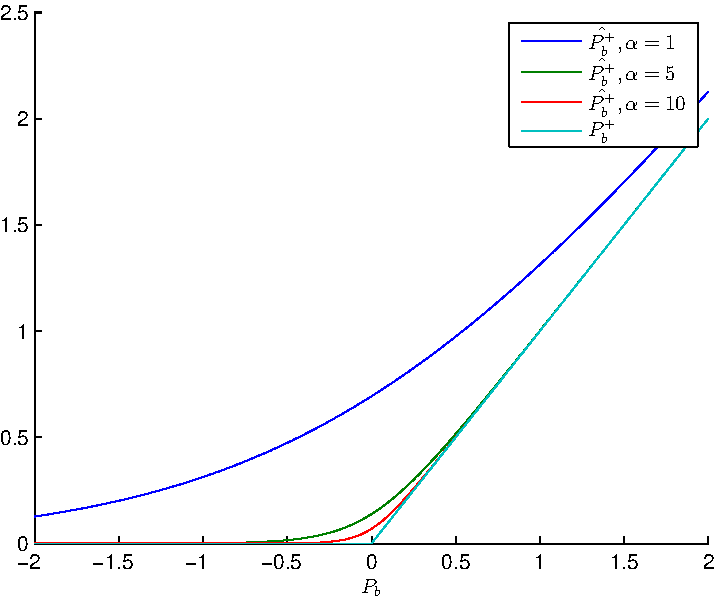
\includegraphics[width = 3in]{cfapprox}
 \caption{$\hat{P_b^+}$ approaches $P_b^+$ as $\alpha$ increases}
 \label{f:Phat}
\end{figure}


\subsection{Comparison with Regenerative Braking Case}
In the presence of regenerative braking, the cost functional for a single wheel can be written as:
\begin{align}
\label{eqn12}
J =  \left(\frac{R_a}{k_t^2}\right)\int_{t_0}^{t_f}u^{2} \; dt + 
\left(\frac{2R_a\mu_f}{k_ek_t}+\frac{k_e}{k_t}\right) \int_{t_0}^{t_f}u\omega_w \; dt + 
\left(\mu_f+\frac{R_a\mu_f^2}{k_e^2}\right) \int_{t_0}^{t_f}\omega_w^{2} \; dt
\end{align}

\noindent For the problem being solved in this paper, where there are no external torques, three reaction wheels, and the initial and final angular velocity of the satellite body is 0, the reaction wheels must have the same angular velocities at the beginning and end of the maneuver. In these circumstances, the second term of equation~\ref{eqn12} integrates to zero.\cite{Marsh2015} Because the reaction wheels are being operated in the vacuum of space, the last term tends to be relatively small compared to the first. Thus, in the presence regenerative breaking, equation \ref{eqn12} reduces to:
\begin{align}
J \approx \left(\frac{R_a}{k_t^2}\right)\int_{t_0}^{t_f}u^{2} \; dt
\end{align}

\noindent which is the $QC$ cost. 

\section{Results}
This section presents optimal control trajectories computed with DIDO for the fixed time, large angle attitude reorientation problem. Optimization is performed with respect to both the $QC$ and $\hat{EEC}$ cost functionals for two different values of reaction wheel moment(s) of inertia (MOI). Figures \ref{f:BWT} and \ref{f:SWT} present these results, while Table~\ref{tab:EECC} provides a comparison of the $EEC$ costs of these maneuvers. The wheel MOI used to compute the solutions in Figure \ref{f:SWT} are the same as that of a commercially available Cubesat reaction wheel \cite{BCTdatasheet}.

\begin{figure}[h!]
\centering
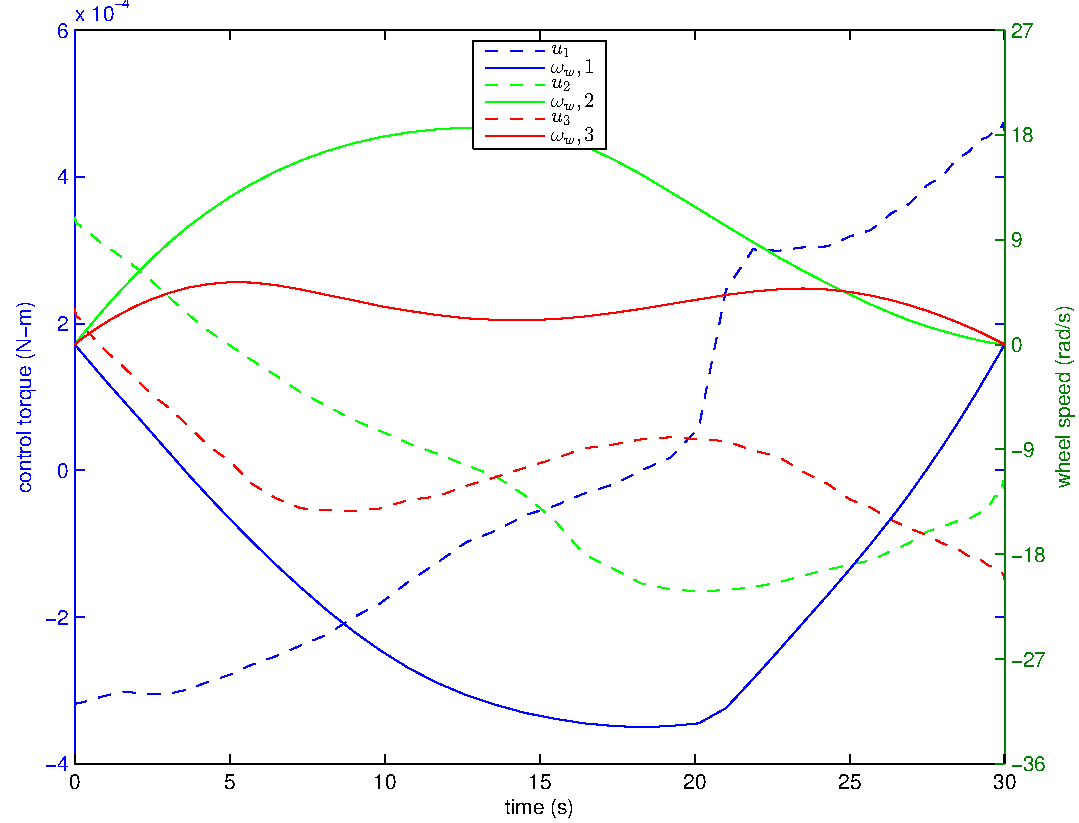
\includegraphics[width = 5.1 in]{figures/3u_master_50N_soln_controls_and_wheel_speeds_cropped.pdf}
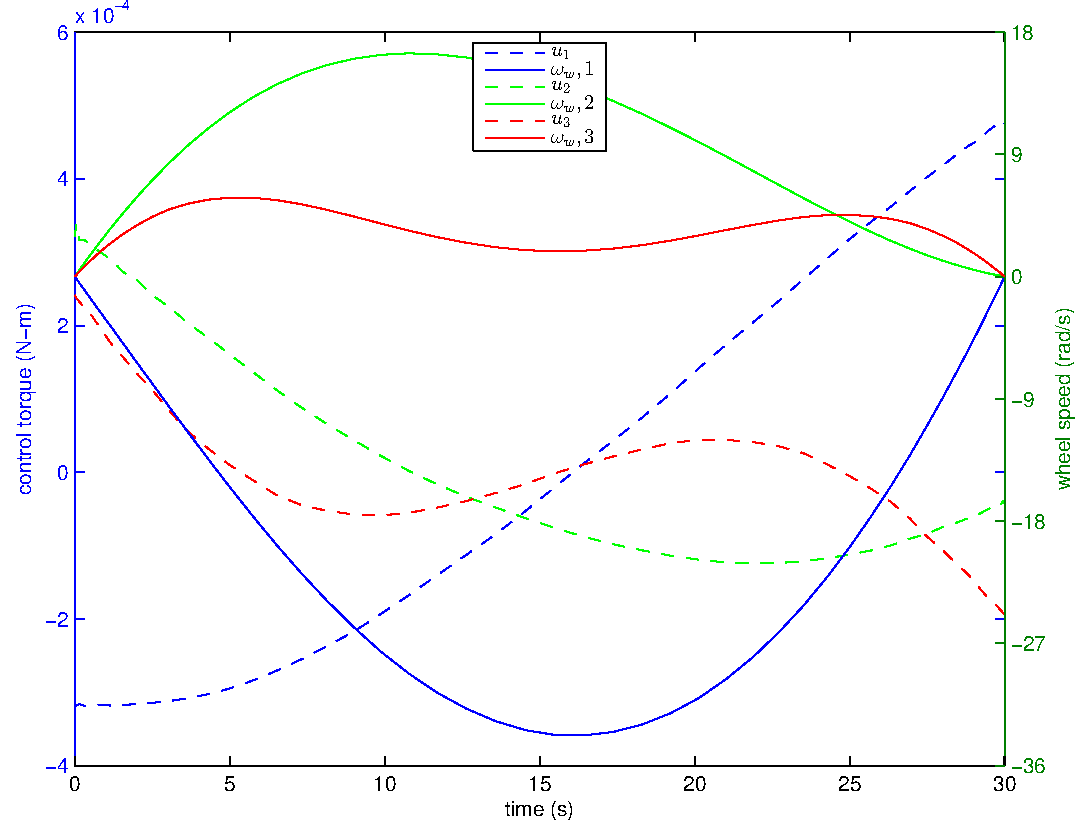
\includegraphics[width = 5.1 in]{figures/3u_u2_50N_soln_controls_and_wheel_speeds_cropped.pdf}
\centering
\caption{Control torques and reaction wheel speeds for optimal energy maneuvers computed with respect to $\hat{EEC}$ (top) and $QC$ (bottom), for a 3U Cubesat with high-MOI reaction wheels ($I_w = 1.0 \times 10^{-4}\; kg \cdot m^2$)}
\label{f:BWT}
\end{figure}

\begin{figure}[h!]
\centering
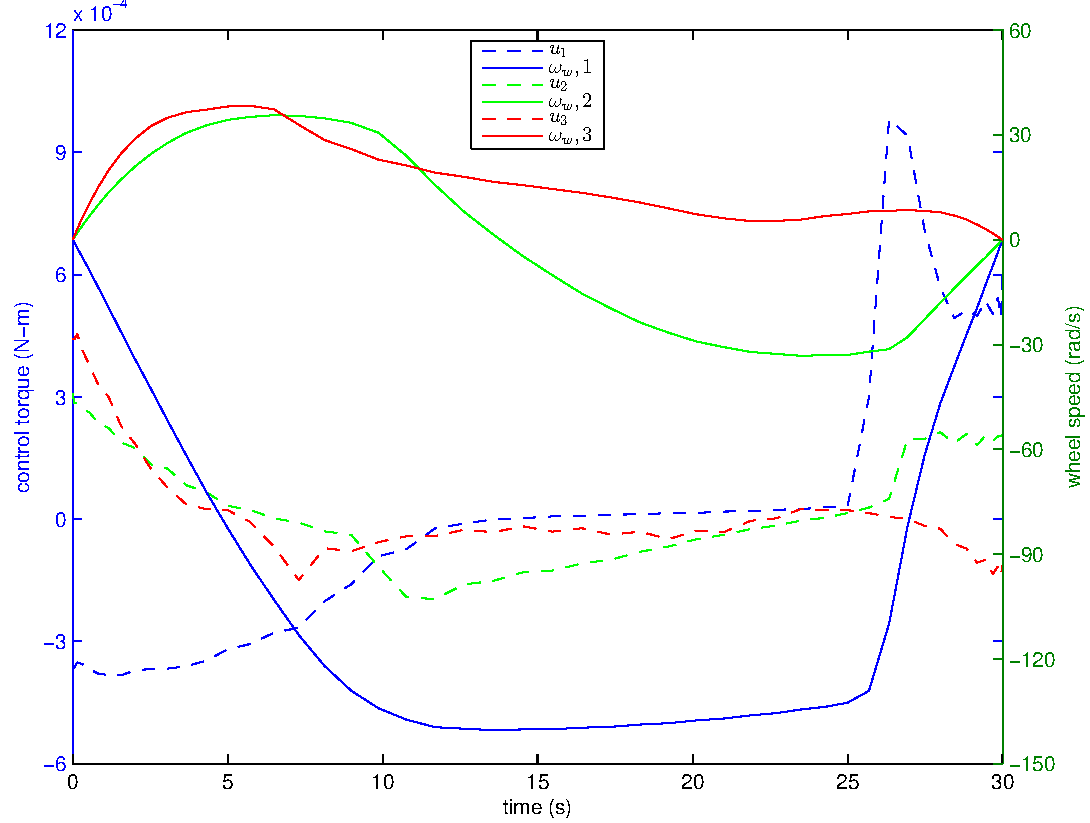
\includegraphics[width = 5.1 in]{figures/3u_master_50N_soln_BC_controls_and_wheel_speeds_cropped.pdf}
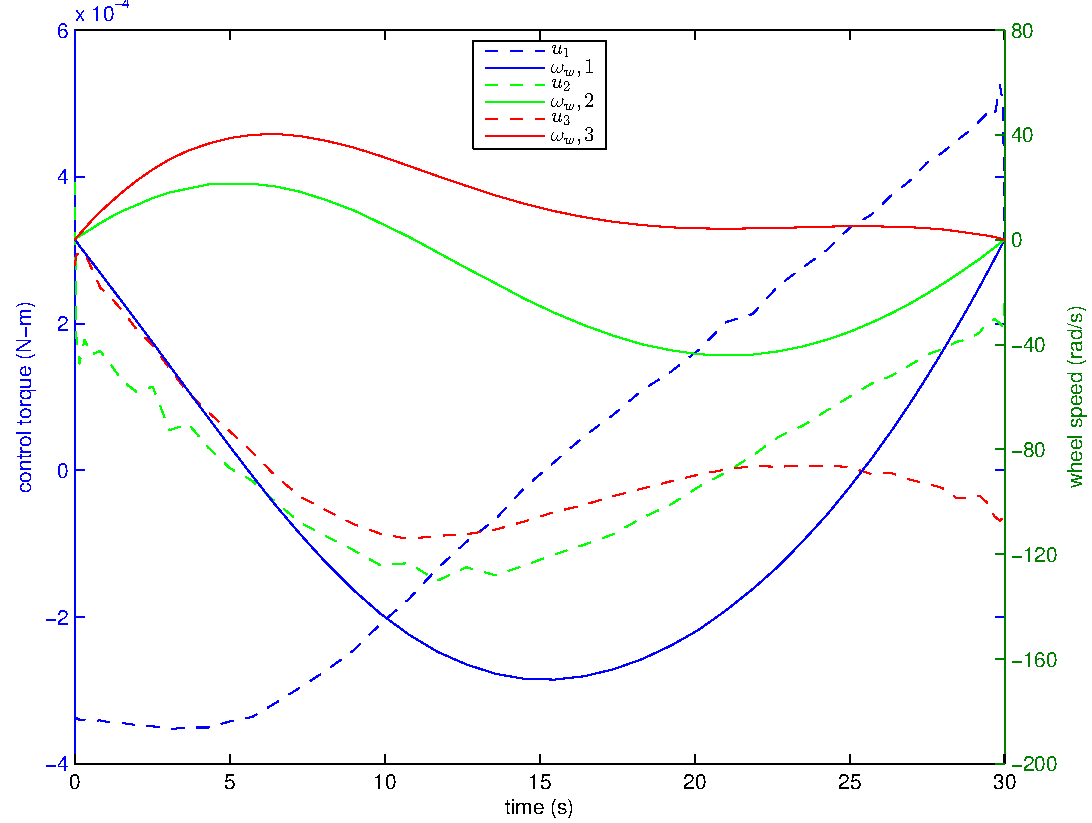
\includegraphics[width = 5.1 in]{figures/3u_u2_50N_soln_BC_controls_and_wheel_speeds_cropped.pdf}
\centering
\caption{Control torques and reaction wheel speeds for optimal energy maneuvers computed with respect to $\hat{EEC}$ (top) and $QC$ (bottom), for a 3U Cubesat with lower-MOI reaction wheels ($I_w = 2.2 \times 10^{-5}\; kg \cdot m^2$).}
\label{f:SWT}
\end{figure}

\begin{table}[h!]
	\fontsize{10}{10}\selectfont
        \centering 
   \begin{tabular}{c | c | c} % Column formatting, 
      \hline 
      Wheel Inertia    & $\hat{EEC}$ solution & $QC$ Solution   \\
      \hline 
      High Inertia      & 0.246 & 0.250  \\
      Low Inertia       & 0.444 & 0.539 \\ 
      \hline
   \end{tabular}
   	       \caption{Summary of $EEC$ costs (Joules).}
	   \label{tab:EECC}
\end{table}

\subsection{Discussion of Results}
The wheels in Figure \ref{f:BWT} have MOI about 5 times larger than those in Figure \ref{f:SWT}. The two trajectories in Figure \ref{f:BWT} are nearly identical, and have the same $EEC$ cost. On the other hand, the solutions in Figure \ref{f:SWT} have significantly different control trajectories, and the $EEC$ cost of the $QC$ solution is over 20$\%$ higher than that of the $\hat{EEC}$ solution. Reaction wheels with smaller MOI have to spin faster than wheels with larger MOI to produce the same angular rate in the satellite body. As $\omega _w$ increases, the second and third terms of equation \ref{eqn7} increase and begin to have a more significant effect on total cost. On the other hand, the first term is agnostic to the wheel velocity (as long as saturation limits are not reached). This is why the $QC$-optimal control trajectories for different wheel MOI are nearly the same.

The cost of the maneuver is approximately twice as high with the low-MOI wheels. For an intuitive explanation of this phenomenon, examine two reaction wheels, $W_1$ and $W_2$, with moments of inertia $J$ and $\alpha J$, respectively. The angular moments and kinetic energies of these wheels are:
\begin{align}
H_1 = J\omega_1 \;, \; \; E_1 = \frac{1}{2}J\omega_1^2 \\
H_2 = \alpha J \omega_2 \;, \; \; E_2 = \frac{1}{2}\alpha J \omega_2^2
\end{align}

\noindent In order for these two wheels to produce the same body rate, they must have the same angular moments:
\begin{align}
J\omega_1 = \alpha J \omega_2 \\
\omega_1 = \alpha\omega_2 \\
E_2 = \frac{1}{2} \alpha J (\frac{\omega_1}{\alpha})^2 \\
E_2 = \frac{1}{2\alpha} J \omega_1^2 \\
\label{eqn20}
E_1 = \alpha E_2
\end{align}

\noindent Equation \ref{eqn20} shows that the kinetic energy in the momentum wheel required to produce a certain body rate grows linearly with decreasing MOI. Because this energy can't be recovered the $EEC$ cost of the same maneuver is higher with lower-MOI wheels.


\section{Conclusion}
The $QC$ is a convenient cost functional for energy optimization in large angle attitude maneuvers; it is well suited to numerical optimization, and it is applicable to a variety of different actuators. Further analysis of the reaction wheel based system reveals that the $QC$ accounts for a significant fraction of the total electrical energy consumed by the system, but that there are other significant terms to consider when the reaction wheel speeds become large, which tends to occur when the MOI of the inertial wheels are small compared to those of the satellite body. Numerical optimization confirms that control trajectories which consume less electrical energy are possible when a more realistic cost functional is passed to the optimization algorithm. In the absence of regenerative breaking, this cost functional is not suited to numerical optimization. A smoothing approximation was introduced, which allowed numerical optimization to be successfully performed. This method is applicable to a class of nonsmooth cost functionals. The utility of this method can be improved through the development of an automated approach to choosing $\alpha$, the factor which determines the curvature of the approximation in the neighborhood of the non-smooth point. 

Further investigations can focus on optimization in a wider variety of scenarios, including operation of the wheels at a non-zero bias, trajectories which involve reaction wheel saturation, and a system with differently sized reaction wheels. Even the $EEC$ functional does not include all loss sources. Efforts should be made to include other loss terms to further the fidelity of the cost functional. Examples include switching and core losses.

The energy costs presented in Table \ref{tab:EECC} are relatively small (on the order of half a joule), which may be negligible for some missions, depending on the frequency of attitude maneuvering, the power produced by the solar panels, and the demands of other subsystems, and energy optimization for those satellites may not be worth the effort. If this is the case, it is likely that the reaction wheels are too large and heavy, and there is ample room for weight savings without violating the energy constraints. Energy optimization at design time will allow designers to use smaller, lighter reaction wheels while conforming to energy constraints, leaving more room for payload.

\section{Acknowledgment}
The authors would like to thank Qi Gong for insightful discussions and review.

\section{Notation}
\begin{table}[h!]
	\fontsize{10}{10}\selectfont
    \caption{Notation}
   \label{tab:notation}
        \centering 
   \begin{tabular}{c r } % Column formatting, 
      \hline 
      $\mathbf{u}$ & Column vector of the torques exerted by the motors  \\
      $\pmb{\omega}_{w}$      & Column vector of reaction wheel speeds W.R.T satellite body \\
      $\pmb{\omega}$       & Body frame angular velocity W.R.T inertial frame, in body coordinates \\
      $\pmb{q}$      & Unit quaternion expressing body frame attitude \\
      $\pmb{x}$ & $\lbrack 
      \pmb{\omega}^T \;\pmb{\omega}_{w}^{T} \; \pmb{q}^{T}
      \rbrack^{T}$\\
      $\pmb{a}_{i}$ & Orientation of spin axis of wheel $i$ w.r.t body frame \\
      $\pmb{I}$ & Inertia tensor of spacecraft with freely rotating wheels \\
      $I_{w,i}$ & Moment of inertia of wheel $i$ about its spin axis \\
      \hline
   \end{tabular}
\end{table}

\section{Appendix: Values used for Optimization}
\label{app:Numerical Values}

\begin{align*}
t_{0} = 0 \; s  \\
t_{f} = 30 \; s \\
\lbrack yaw, pitch, roll\rbrack_{0} = \lbrack 0, 0, 0\rbrack rad \\
\pmb{u}_{U} = -\pmb{u}_{L} = \begin{bmatrix}3 & 3 & 3 \end{bmatrix}^{T} \times 10^{-3} \; N \cdot  m \\
\pmb{\omega}_{w,U} = -\pmb{\omega}_{w,L} = \begin{bmatrix} 650 & 650& 650 \end{bmatrix}^{T} \; rad/s \\
I_{w,1} = I_{w,2} = I_{w,3} = 
\begin{cases}
1.0 \times 10^{-4} \; kg \cdot m^2, & \text{Figure \ref{f:BWT}} \\
2.2 \times 10^{-5} \; kg \cdot m^2, & \text{Figure \ref{f:SWT}}
\end{cases} \\
\pmb{I} = \begin{bmatrix}
248 & 0.21 & 0.61 \\
0.21 & 248 & 0.61 \\
0.61 & 0.61 2 & 49 \\
\end{bmatrix} \times 10^{-4} \; kg \cdot m^{2}\\
\pmb{a}_1 = \begin{bmatrix}
1 \\ 0 \\ 0
\end{bmatrix} \; , \;
\pmb{a}_2 = \begin{bmatrix}
0 \\ 1 \\ 0
\end{bmatrix} \; , \;
\pmb{a}_3 = \begin{bmatrix}
0 \\ 0 \\ 1
\end{bmatrix} \;
\end{align*}


\bibliographystyle{AAS_publication}   % Number the references.
%\bibliography{C:/Users/Dmitriy/Documents/library,
\bibliography{C:/Users/Dmitriy/Documents/References/library,C:/Users/Dmitriy/Documents/References/harleigh}   % Use references.bib to resolve the labels.



\end{document}
